\documentclass[12pt]{article}
\usepackage[utf8]{inputenc}
\usepackage{amsmath,amssymb}
\usepackage{unicode-math}
\usepackage[T2A]{fontenc}
\usepackage[russian]{babel}
\usepackage{graphicx}
\usepackage{subfigure}
\usepackage{subcaption}


\DeclareGraphicsExtensions{.pdf,.png,.jpg}
\usepackage{hyperref}
\usepackage{wrapfig}
\usepackage[left=20mm, top=20mm, right=10mm, bottom=20mm]{geometry}

\usepackage{amsmath} 
\usepackage{amsfonts} 
\usepackage{amssymb} 
\usepackage{wasysym} 
\usepackage{fancyhdr}

\pagestyle{fancy}
\fancyhf{}
\lhead{Семинар 1. Тепловое излучение}
\rhead{\textit{Клименок К.Л., МФТИ 2020}}
\rfoot{\thepage}



\begin{document} 
\title{\textbf{Семинар 1. Предпосылки квантовой механики. Законы излучения абсолютно черного тела.}}
\author{\textbf{Клименок Кирилл Леонидович}}
\date{03.09.2020}
\maketitle
\section{Теоретическая часть}
\subsection{Предпосылки возникновения "неклассической" теории}
За прошлые 2 года обучения мы с вами рассмотрели основные разделы классической физики, а именно механику, термодинамику, электричество и оптику, и по состоянию на текущий момент, мы остановились примерно в том же месте, что и ученые конца 19 века. Кажется, что основные законы существования мира известны и можно смело с их помощью объяснять все происходящие вокруг явления. К сожалению, это не совсем так и вот ряд проблем с которыми не очень понятно, что делать.
\paragraph{Модель атома Резерфорда}
Опыт Резерфорда по рассеянию альфа-частиц на атомах тонкой фольги известен нам еще со школы, но стоит напомнить его основной вывод: положительный заряд и почти вся масса атома сосредоточена в его ядре, а характерные масштабы ядра много меньше масштабов атома. Но в сумме атом нейтрален, а это значит, что электроны "вращаются" вокруг ядра по каким-то траекториям. И вот оно противоречие: если электрон движется по финитной орбите к поле ядра, то у него есть ускорение и он должен излучать что-то, как и любая уважающая себя заряженная частица, и в конечном итоге просто упасть на ядро и все. Этого не происходит в реальном мире. Как это объяснить мы рассмотрено в семинаре 6.
\paragraph{Линейчатые спектры излучения и поглощения атомов} 
При исследовании спектров излучения или поглощения различных материалов оказалось, что некоторые из них излучают или поглощают только определенные длины волн, а не все возможные. Это тоже проблема, у которой нет нормального классического обоснования. Ее решение тесно связано с первой проблемой и она тоже будет обсуждена в 6 семинаре
\paragraph{Внешний фотоэффект} 
Явление при котором свет выбивает электроны из катода вакуумной лампы было известно еще с 1839 года, но когда в нем начали разбираться, оказалось, что результаты противоречат классическом представлению. Казалось бы, чем больше интенсивность света, тем больше фототок независимо от длины волны, но в реальности есть строгая граница по длине волны (красная граница фотоэффекта), когда фототок вообще прекращается, с какой интенсивностью на фотокатод бы не светили. Это проблема будет обсуждаться нами во 2 семинаре. 
\paragraph{Равновесное тепловое излучение}
На этом явлении мы остановимся подробнее именно сегодня и обсудим что же здесь не так.
\subsection{Модель равновесного теплового излучения абсолютно твердого тела}
Что-то слишком умный заголовок получается, не находите? Давайте разберемся что же это за зверь такой и с чем его едят. Во-первых с классической точки зрения, почему тело излучает? Все просто -- есть заряженные частиц, они движутся с ускорением, вот нам и излучение. Хорошо, но с чего вдруг они движутся? Еще проще  -- тепловое движение. А если вспомнить, что вообще-то тела состоят из молекул, которые могут быть еще и полярными, то все вообще встает на свои места. Или еще нет? Если так, вот пример того, где мы это тепловое излучение можем видеть: разогреем железку до достаточно высокой температуры, около 500 градусов Цельсия, она начнет светиться красным, будем повышать температуру дальше, получим желтый, а затем и белый цвет свечения. Или еще более жизненный пример -- обычная лампа накаливания. Температура вольфрамовой нити там около 2500 К, именно поэтому она и светится. И последний пример это банально мы с вами. Если вспомнить актуальную пандемию и измерение температуры на входе в любые учреждения, то принцип работы термометра там точно такой же, правда мы с вами излучаем не в видимом, а инфракрасном диапазоне.
\begin{figure}[h]
    \centering
    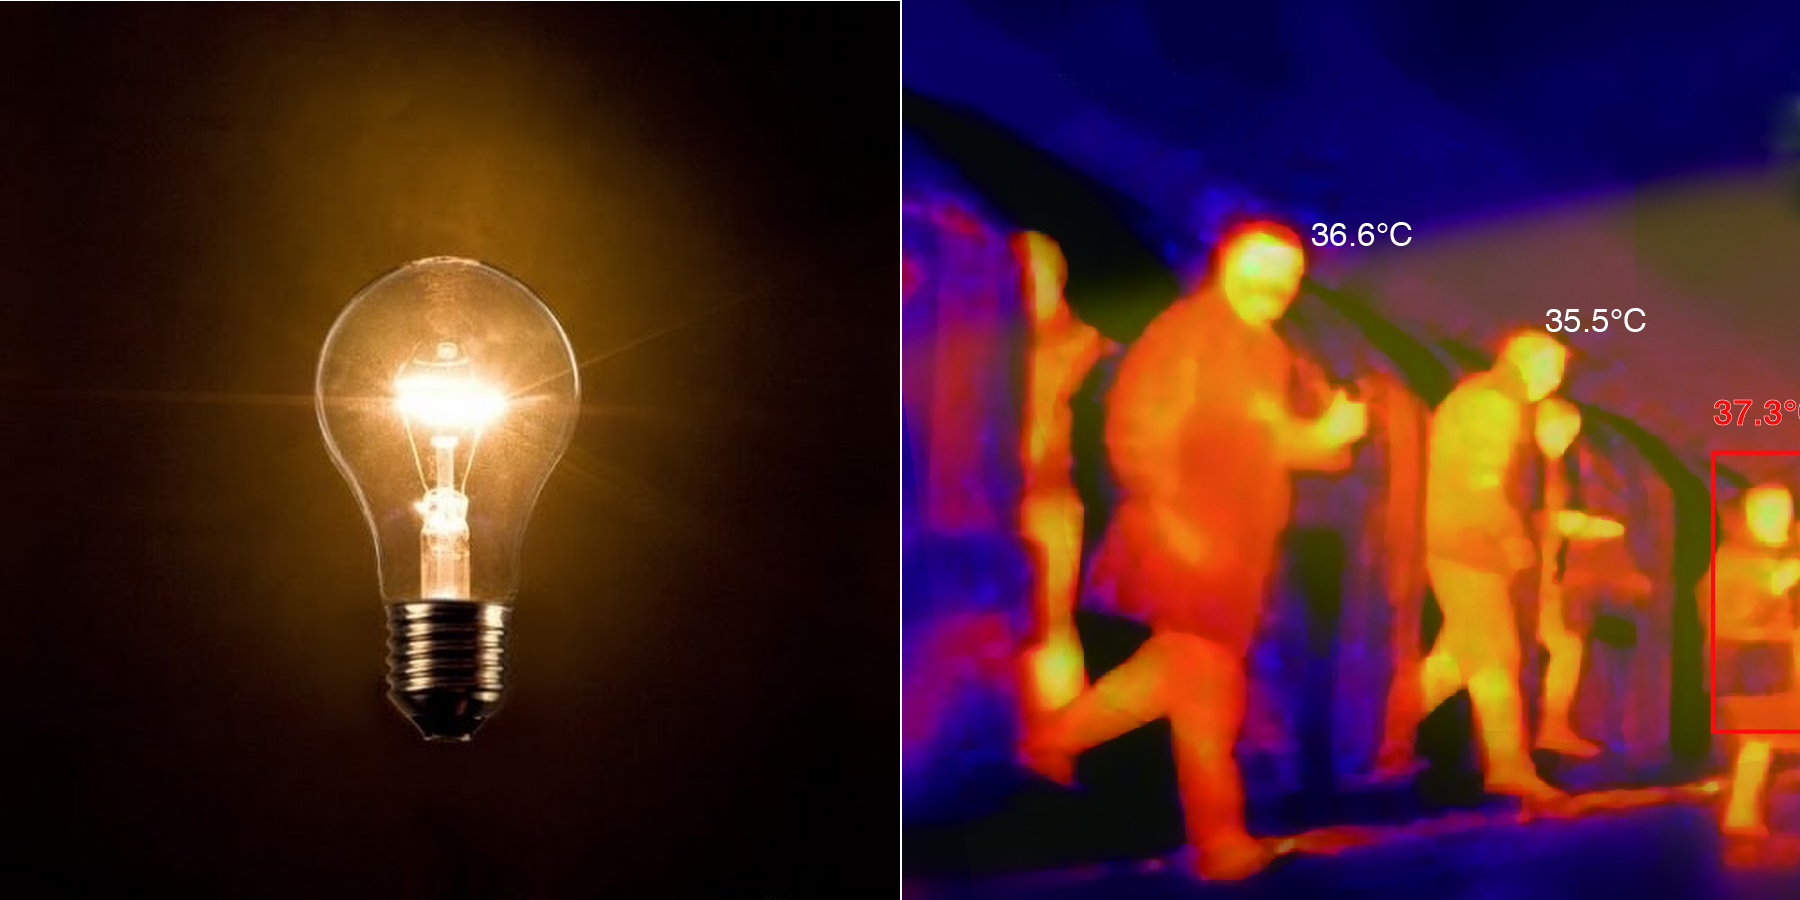
\includegraphics[width=\textwidth,height=\textheight,keepaspectratio]{Seminar_01/pics/pic_01.png}
    \caption{Примеры равновесного теплового излучения}
    \label{fig:sem_01_radiation_examples}
\end{figure}
\\
Теперь давайте разберемся с абсолютно черным телом или АЧТ. Во-первых что это? АЧТ -- тело, которое поглощает всё падающее излучение и равновесным образом переизлучает его. Для того, чтобы казаться умнее введем несколько характеристик тела по отношению к излучению: 
\begin{itemize}
    \item Поглощательная способность: $a(\omega) = \dfrac{W_{\text{погл}}}{W_{\text{пад}}}$ -- отношение всей поглощенной энергии ко всей падающей энергии излучения, $a_{\text{АЧТ}} = 1$
    \item Излучательная способность: $b(\omega) = \dfrac{W_{\text{изл}}}{W_{\text{АЧТ, изл}}}$ -- отношение всей энергии, излучаемой телом, ко всей энергии излучаемым АЧТ, $b_{\text{АЧТ}} = 1$
    \item Отражательная способность: $1 - a(\omega)$ -- какая доля энергии отражается от тела
\end{itemize}
Из основного, что по этим характеристикам нужно вынести -- поглощательная способность всегда равна излучательной, даже если это какое-то обычное тело, а не абсолютно черное. Предлагаю вам самостоятельно подумать, почему если это не так, то можно собрать вечный двигатель.
\\
Теперь построим простейшую модель абсолютно черного тела. Она представляет из себя полую камеру с нагретыми стенками, которые излучают и поглощают свет. На самом деле идея такой камеры чем-то очень сильно схожа с обычным идеальным газом в сосуде, только там частицы упруго отражаются от стенок, а здесь поглощаются и переизлучаются обратно. Это представление упростит нам жизнь, потому, что мы в явном виде из такой аналогии получим все что нам надо. Оговоримся, что полость большая, все излучение изотропно и дело происходит в тепловом равновесии. Также площадка, через которую излучение проходит наружу, мала и не влияет ни на что. 
\\
\begin{figure}[h]
    \centering
    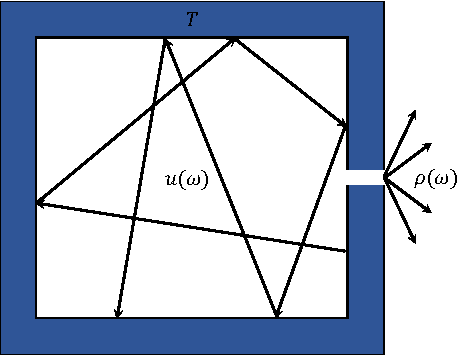
\includegraphics[scale=1.5]{Seminar_01/pics/pic_02.pdf}
    \caption{модель абсолютно черного тела. $T$ -- температура до которой нагреты стенки, $u(\omega)$ -- плотность энергии излучения внутри полости, $\rho(\omega)$ -- спектральная плотность излучения с единицы площади}
    \label{fig:sem_01_abb_model}
\end{figure}
\\
Введем 2 характеристики, которые мы будем использовать для описания этого излучения, а именно плотность энергии излучения внутри полости $u(\omega) = \dfrac{dE}{d\omega}$ и спектральную плотность изучения, которую видит наблюдатель с единицы площади $\rho(\omega) = \dfrac{dE/d\omega}{dSdt}$. А теперь чтобы их связать, нужно всего лишь проинтегрировать по времени и по всему телесному углу, из которого приходит излучение в отверстие. Ничего не напоминает? Мы делали подобное для частиц, которые бьются о единичную площадку стенки, когда говорили о распределении Максвелла во 2 семестре, только $u(\omega)$ станет здесь по сути концентрацией, a $\rho(\omega)$ - тем самым потоком на стенку. И для связи нужно лишь определиться со скоростью, но тут все просто у излучения это скорость света. В результате имеем:
\begin{equation}
    \rho(\omega) = \dfrac{cu(\omega)}{4}
\end{equation}
Осталось разобраться с последним вопросом, а именно, сколько вообще волн в нашем излучении попадает в диапазон частот $d\omega$. вот тут нам понадобится вспомнить одну из самых плохо запоминаемых тем 3 семестра, а именно резонаторы. Я надеюсь, что что-то еще всплывает в памяти, что не всякую волну можно запихать в нашу коробку из-за граничных условий (нуля поля $E$ на стенках). Тогда для простоты будем считать коробку кубической со стороной $L$ и ограничения на все возможные волновые вектора можно записать как:
\begin{gather*}
    k_x = \dfrac{\pi A}{L}, k_y = \dfrac{\pi B}{L}, k_z = \dfrac{\pi C}{L}; A, B, C\in \mathbb{N}\\
    \omega^2 = k^2c^2 \Rightarrow A^2+B^2+C^2 = \dfrac{\omega^2L^2}{c^2\pi^2}
\end{gather*}
То есть, если мы нарисуем пространство состояний для всех возможных волн то, поверхность постоянной частоты будет сферой, а для подсчета всех волн на интервале частот $d\omega$ будет пропорционально сферическому слою, в который попадет некоторое количество состояний. Единственная оговорка, про которую надо сказать, что характерные частоты, на которое мы смотрим, вообще все возможные, и поэтому дискретные точки в этом пространстве мы можем просто заменить непрерывным распределением. тогда:
\begin{equation}
    dN = \dfrac{1}{8}4\pi R^2 \dR \sim \omega^2d\omega \Rightarrow \dfrac{dN}{d\omega} \sim \omega^2
\end{equation}
\\
\begin{figure}[h]
    \centering
    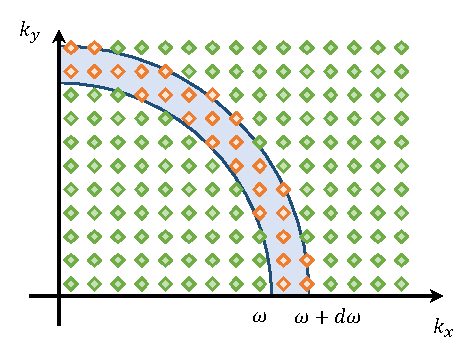
\includegraphics[scale=1.5]{Seminar_01/pics/pic_03.pdf}
    \caption{Двумерный срез пространства всех возможных существующих в резонаторе волн. Точки соответствуют разрешенным состояниям ($A=1, 2, ...; B = 1, 2, ...$), дуги окружностей -- поверхность постоянной частоты. Те волны, которые попдают в интервал частот $d\omega$ выделены красным}
    \label{fig:sem_01_dN_domega}
\end{figure}
\\
Тогда, по теореме о равнораспределении по степеням свободы, каждая волна имеет $kT$ энергии с 2 поляризациями иесли мы попытаемся посчитать всю энергию теплового излучения, то есть проинтегрировать: 
\begin{equation*}
    E = \int\limits_{0}^{+\infty} 2kT\dfrac{dN}{d\omega}d\omega \rightarrow \infty
\end{equation*}
мы получим расходимость. Эта проблема называется "ультрафиолетовой катастрофой", дело в том, что в реальности конечно нет никаких бесконечных энергий и при измерении спектральной плотности именно в зоне ультрафиолетовых волн начиналась расходимость классической теории и эксперимента.
\subsection{Формула Планка}
В чем же заключался шикарный подгон Планка для решения этой проблемы. Он решил, что при колебаниях электромагнитного поля на данной частоте может быть запасено только целое число квантов колебаний $E_n =n \hbar \omega$. Тогда в тепловом равновесии все должно быть распределено по Больцману и средняя энергия для излучения на данной частоте уже не просто $kT$, а вот это:
\begin{equation*}
    \langle E \rangle = \dfrac{\sum\limits_{n=0}^{\infty} E_n \exp{\left(-\dfrac{n\hbar \omega}{kT}\right)}}{\sum\limits_{n=0}^{\infty} \exp{\left(-\dfrac{n\hbar \omega}{kT}\right)}} = \dfrac{\hbar \omega}{\exp{\left(\dfrac{\hbar \omega}{kT}\right)} - 1}
\end{equation*}
Честный расчет этих сумм можно также посмотреть во 2 семестре в теме о статсуммах, или посчитать самостоятельно, если увидеть убывающую геометрическую прогрессию. Давайте исследуем это выражение для случаем, когда энергия кванта излучения много больше и много меньше тепловой:
\begin{align*}
    \hbar \omega \ll kT &\Rightarrow \langle E \rangle = kT \text{ классический предел} \\
    \hbar \omega \gg kT &\Rightarrow \langle E \rangle = \hbar \omega  \exp{\left(-\dfrac{\hbar \omega}{kT}\right)} \text{ случай высоких частот}
\end{align*}
Как видно из этого выражения, никаких проблем с расходимостью при больших частотах больше нет, ведь там все спадает по экспоненте. Теперь мы можем спокойно записать спектральную плотность излучения, или другими словами, формулу Планка:
\begin{gather}
\label{eq:sem_01_plank}
    \rho(\omega)d\omega = \dfrac{\hbar \omega^3}{4\pi^2c^2\left[ \exp{\left(\dfrac{\hbar \omega}{kT}\right)} - 1\right]}d\omega\\
    \rho(\lambda) d\lambda = \dfrac{\pi h c^2}{\lambda^5\left[ \exp{\left(\dfrac{\hbar c}{\lambda kT}\right)} - 1\right]}d\lambda
\end{gather}
отличия степеней частоты и длины волны связано с тем, что мы заменяем не только саму переменную, но и дифференциал по которому мы будем интегрировать.


\begin{figure}[h]
    \centering
    \begin{minipage}{0.5\textwidth}
        \centering
        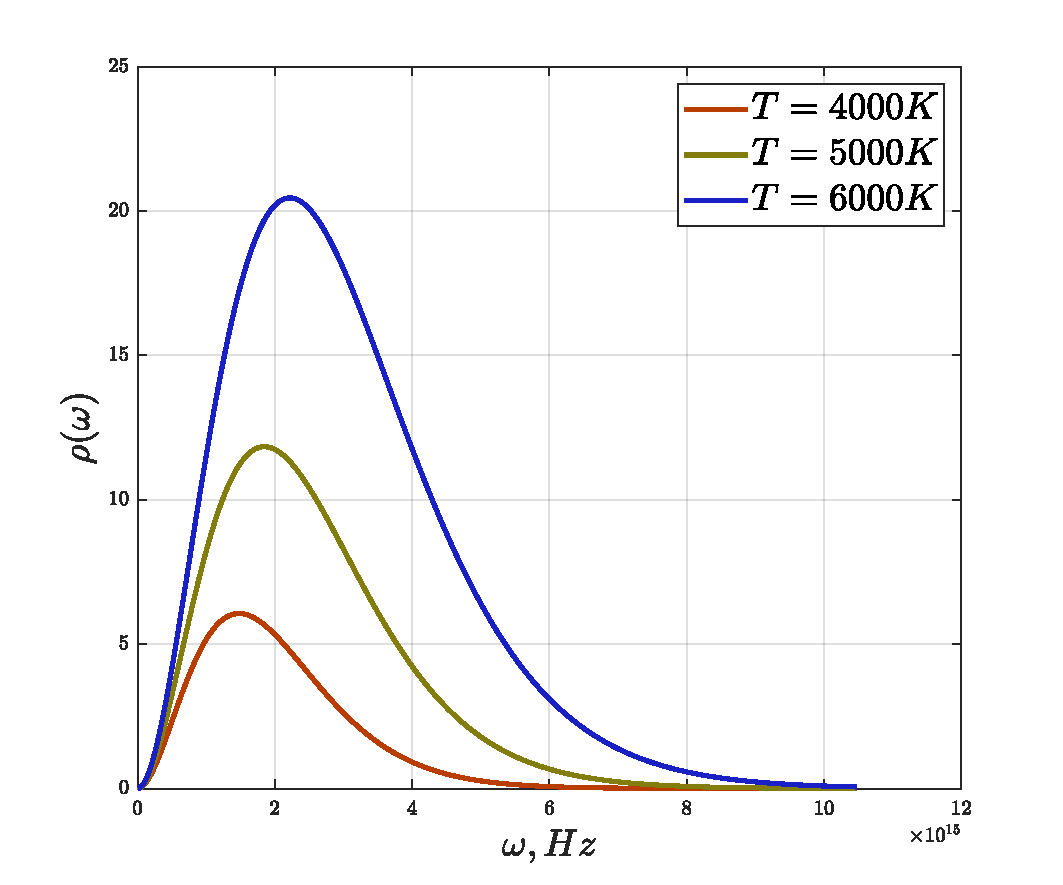
\includegraphics[width=1.0\textwidth]{Seminar_01/pics/pic_04_left.pdf}
    \end{minipage}\hfill
    \begin{minipage}{0.5\textwidth}
        \centering
        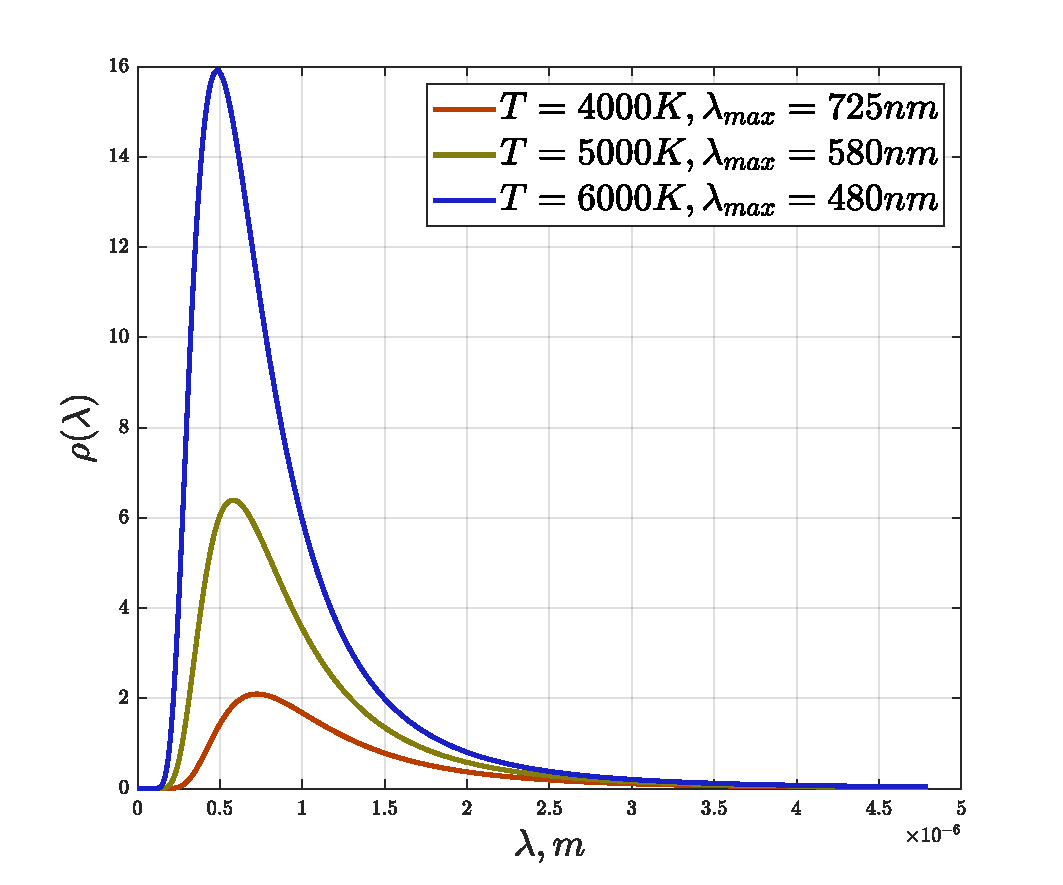
\includegraphics[width=1.0\textwidth]{Seminar_01/pics/pic_04_right.pdf}
    \end{minipage}
    \caption{Формулы Планка для разных температур. Слева представлена зависимость спектральной плотности излучения от циклической частоты, справа -- от длины волны. Цвет линий соответствует характерной длине волны с максимальной спектральной плотностью}
    \label{fig:sem_01_plank_func}
\end{figure}

Построим графики этих функций для разных температур, см. рисунок \ref{fig:sem_01_plank_func}. Как видно из рисунка у них есть максимум, по которому можно легко оценить характерную длину волны, которое излучает тело данной температуры. При этом с ее изменением это максимум смещается. Это смещение называют законом смещения Вина и оно описывается уравнением:
\begin{equation}
\label{eq:sem_01_vin}
    \lambda_{max} = \dfrac{2.9 \cdot 10^6}{T \text{[K]}} \text{ нм}
\end{equation}
И последнее по теории, что нам здесь нужно выяснить, это полная мощность излучения, или интегральная светимость. Для этого просто проинтегрируем функцию Планка по всем частотам и получим закон Стефана-Больцмана:
\begin{equation}
\label{eq:sem_01_stefan_boltzman}
    P_{total} =\int\limits_{0}^{\infty}\rho(\omega)d\omega = \int\limits_{0}^{\infty}\dfrac{\hbar \omega^3}{4\pi^2c^2\left[ \exp{\left(\dfrac{\hbar \omega}{kT}\right)} - 1\right]}d\omega = \sigma T^4
\end{equation}
Здесь $\sigma = 5.67 \cdot 10^{-8} \dfrac{\text{Вт}}{\text{м}^2 \text{К}^4}$ -- постоянная Стефана-Больцмана

\section{Практическая часть}
\subsection{Задача 0-1-1}
\label{task_011}
\paragraph{Условие}
Вследствие повышения температуры положение максимума спектральной  энергетической  светимости  абсолютно  черного  тела  переместилось  с  2 мкм на 1 мкм. Во сколько раз изменилась его интегральная энергетическая светимость?
\paragraph{Решение}
Это задачка на подстановку в 2 формулы, закон смещения Вина (\ref{eq:sem_01_vin}) и закон Стефана-Больцмана (\ref{eq:sem_01_stefan_boltzman}). Из первого найдем отношение температур и зная его найдем отношение светимостей: 
\begin{equation*}
    \dfrac{T}{T_0} = \dfrac{\lambda_0}{\lambda} \Rightarrow \dfrac{P}{P_0} = \dfrac{T^4}{T^4_0} = \dfrac{\lambda^4_0}{\lambda^4} = 2^4 =16 
\end{equation*}
\subsection{Задача 0-1-2}
\label{task_012}
\paragraph{Условие}
Оценить давление теплового излучения во внутренней области Солнца, где температура равна $1.3\cdot 10^7$ К?
\paragraph{Решение}
Здесь нам нужно что-то знать про давление фотонного газа. Естественно,  если покопаться в термодинамических потенциалах, подифференцировать их и немного поколдовать, то в явном виде можно получить формулу для давления. Естественно, здесь мы не будем этим заниматься, а максимально упростим себе жизнь путем аналогии с идеальным газом. Для него из молекулярно кинетической теории известны формулы для давления:
\begin{equation*}
    p=\dfrac{1}{3}nm\langle v^2\rangle = \dfrac{2}{3} n \langle E \rangle
\end{equation*}
Здесь явно видно, что давление, это ничто иное как объемная плотность энергии, а коэффициент, который появляется в формуле получается из 3-мерной геометрии нашего пространства. Тогда просто по аналогии с этой формулой давление фотонного газа выражается через объемную плотность энергии $u(\omega)$ с коэффициентом $1/3$. Теперь можно спокойно выписывать все, что необходимо:
\begin{equation*}
    p=\int\limits_0^{+\infty}\dfrac{1}{3}u(\omega) = \int\limits_0^{+\infty}\dfrac{4}{3}c\rho(\omega) = \dfrac{4}{3}c\sigma T^4 = 6.5\cdot 10^{29} \text{ Па}
\end{equation*}
\subsection{Задача 1.22}
\label{task_122}
\paragraph{Условие}
Спектр излучения космического рентгеновского источника соответствует спектру АЧТ. Максимум плотности излучения соответствует $\lambda_{max} = 2$ \AA, а суммарная по спектру плотность потока на Земле равна $j = 10^{-11} \text{ Вт}/\text{см}^2$. Расстояние от источника до Земли $L = 1.3\cdot 10^4$ световых лет. Оценить диаметр источника. 
\paragraph{Решение}
Это задача на банальный закон сохранения энергии. С одной стороны запишем какую энергию излучает со своей поверхности и приравняем это той энергии, которая оказывается на сфере с радиусом $L$. А максимальная длина волны нужна для того, чтобы найти характерную температуру источника:
\begin{gather*}
    \sigma T^4 \cdot 4\pi\left( \dfrac{D}{2}\right)^2 = j\cdot4\pi L^2 \\
    T = \dfrac{0.29 \text{ \AA}}{\lambda_{max}} \approx 1.5 \cdot 10^7 K
\end{gather*}
Окончательно $D\approx15.5$ км
\subsection{Задача 1.23}
\label{task_123}
\paragraph{Условие}
АЧТ подвешено в вакуумной установке так, что через оптическое окно на него падает солнечный свет. Если стенки установки охладить до температуры $T_{\text{ст1}} = 77 $ К, то тело будет иметь температуру $T_{1} = 275 $ К. Какова будет температура тела $T_2$, если $T_{\text{ст2}} = 295 $ К.
\paragraph{Решение}
Разберемся с установкой. Абсолютно черное тело с некоторой температурой подвешено в вакуумной камере, оно за счет обмена излучением взаимодействует со стенками. Помимо прочего, есть еще и поток излучения от Солнца $\Phi$, который тоже надо учитывать. С учетом теплового равновесия эти потоки, которые падают на тело надо приравнять потоку, который тело испускает:
\begin{gather*}
    S_{\text{тела}}\sigma T^4_{\text{ст1}} + \Phi = S_{\text{тела}}\sigma T^4_1\\
    S_{\text{тела}}\sigma T^4_{\text{ст2}} + \Phi = S_{\text{тела}}\sigma T^4_2\\
\end{gather*}
Вычтем из одного из уравнений другое и получим выражение для $T_2$:
\begin{equation*}
    T_2^4 = T_1^4 + T^4_{\text{ст2}} - T^4_{\text{ст1}} = 340 K
\end{equation*}
\subsection{Задача 1.38}
\label{task_138}
\paragraph{Условие}
Напряжение в сети возросло на 5 \%. На сколько процентов увеличится освещенность, создаваемая вакуумной лампой накаливания с температурой нити $T = 1500$ К на длине волны 500 нм. Нить можно считать абсолютно черны телом, рассмотреть случай когда $R(T) = const$ и $R(T) = R_0 + \alpha (T - T_0)$
\paragraph{Решение}
Для начала сделаем общие для этих случаев выкладки. Первое, что от нас хотят? Освещенность на определенной длине волны, это просто $\rho(\lambda)$, с этим и будем работать. Второе, я не хочу тянуть за собой всю формулу Планка и попытаюсь ее упростить в зависимости от значения показателя экспоненты. Для этого сравним $hc/\lambda \sim 10^{-19}$ и $kT\sim10^{-21}$. Видно, что случай существенно квантовый и экспонента забьет единичку. Тогда:
\begin{equation*}
    \rho(\lambda) \sim \exp{\left(-\dfrac{hc}{\lambda kT} \right)} \Rightarrow \ln{\rho(\lambda)} = -\dfrac{hc}{\lambda kT} \Rightarrow \dfrac{\Delta \rho}{\rho} = \dfrac{hc}{\lambda kT} \cdot \dfrac{\Delta T}{T}
\end{equation*}
То есть для того, чтобы решить задачу нужно лишь по относительному изменению напряжения найти относительной изменение температуры, которое повлечет измерение интегральной светимости лампы. Делается это очень просто -- мощность подаваемая на лампу меняет излучаемую мощность. Запишем эту пропорциональность: $\dfrac{V^2}{R} \propto T^4$. Тогда:
\begin{gather*}
    \text{Случай } R(T) = const \Rightarrow V^2 \propto T^4 \Rightarrow 2\dfrac{\Delta V}{V} = 4\dfrac{\Delta T}{T}\\
    \text{Случай } R(T) \propto T \Rightarrow V^2 \propto T^5 \Rightarrow 2\dfrac{\Delta V}{V} = 5\dfrac{\Delta T}{T}\\
\end{gather*}
Именно эти соотношения и надо поставить в полученную в начале формулу
\subsection{Комментарии к задачам из задания}
\paragraph{Нулевки} Решены, \hyperref[task_011]{см.}
\paragraph{Задача 1.22} Решена, \hyperref[task_122]{см.}
\paragraph{Задача 1.26} Землю здесь вполне спокойно можно считать АЧТ и просто записать баланс энергий -- сколько пришло от Солнца (попало на Землю) и сколько излучилось с поверхности Земли
\paragraph{Задача 1.30} Закон Стефана-Больцмана в явном виде
\paragraph{Задача 1.38} Решены, \hyperref[task_138]{см.}
\paragraph{Задача 1.44} Вывод закона Стефана-Больцмана, но не для всех частот, а только для некоторых. Интеграл, который там получится можно взять численно в вольфраме или забить и оценить его.
\paragraph{Задача 1.50} Решена в задачнике плюс отсылки на прошлый семестр. Посмотрим как кто помнит оптику


\end{document}
